\ifx\allfiles\undefined

	% 如果有这一部分另外的package,在这里加上
	% 没有的话不需要
	
	\begin{document}
\else
\fi

    \chapter{运输规划}
    如果有若干个产地,同时又有若干个销售地。那么,根据已有的交通网,应如何制定“将产品从产地运到销售地”的调运方案,使总的运输费用最少,或运输路线最短?运筹问题的数学模型就是运输规划模型。事实上,运输规划是一类特殊的线性规划。
    \section{运输问题}
    \subsection{产销平衡}
    \begin{exbox}{\textbf{产销平衡的运输问题}}
    例\textbf{例}:\ 已知有 \( m \) 个工厂 \( A_{i} \left( i = 1, 2, \ldots, m \right) \),其供应量(产量)分别为 \( a_{i} \left( i = 1, 2, \ldots, m \right) \),有 \( n \) 个销售地 \( B_{j} \left( j = 1, 2, \ldots, n \right) \),其需要量分别为 \( b_{j} \left( j = 1, 2, \ldots, n \right) \)。从 \( A_{i} \) 到 \( B_{j} \) 运输单位物资的运价(单价)为 \( c_{ij} \left( i = 1, 2, \ldots, m; j = 1, 2, \ldots, n \right) \)。
假设总产量等于总销量,且\textbf{产销是平衡的},其数据如表 3.1 所示。
\begin{table}[H] % 使用 H 强制放置位置
    \centering
    \renewcommand{\arraystretch}{1.5} % 调整行高
    \begin{tabular}{|c|c|c|c|c|c|}
        \hline
        \multirow{2}{*}{产品} & \multicolumn{4}{c|}{销量} & \multirow{2}{*}{产量} \\ \cline{2-5}
        & $B_1$ & $B_2$ & $\cdots$ & $B_n$ & \\ \hline
        $A_1$ & $c_{11}$ & $c_{12}$ & $\cdots$ & $c_{1n}$ & $a_1$ \\ \hline
        $A_2$ & $c_{21}$ & $c_{22}$ & $\cdots$ & $c_{2n}$ & $a_2$ \\ \hline
        $\vdots$ & $\vdots$ & $\vdots$ & $\ddots$ & $\vdots$ & $\vdots$ \\ \hline
        $A_m$ & $c_{m1}$ & $c_{m2}$ & $\cdots$ & $c_{mn}$ & $a_m$ \\ \hline
        销量 & $b_1$ & $b_2$ & $\cdots$ & $b_n$ & \\ \hline
    \end{tabular}
    \caption{相关数据表}
\end{table}


\textbf{解}:\ 如采用 $x_{ij}$ 表示从 $A_i$ 到 $B_j$ ($i=1,2,\cdots,m; j=1,2,\cdots,n$) 的运量,则么在产销平衡的情况下,要求供给总量等于最小的调运方式。
\begin{figure}[H]
    \centering
    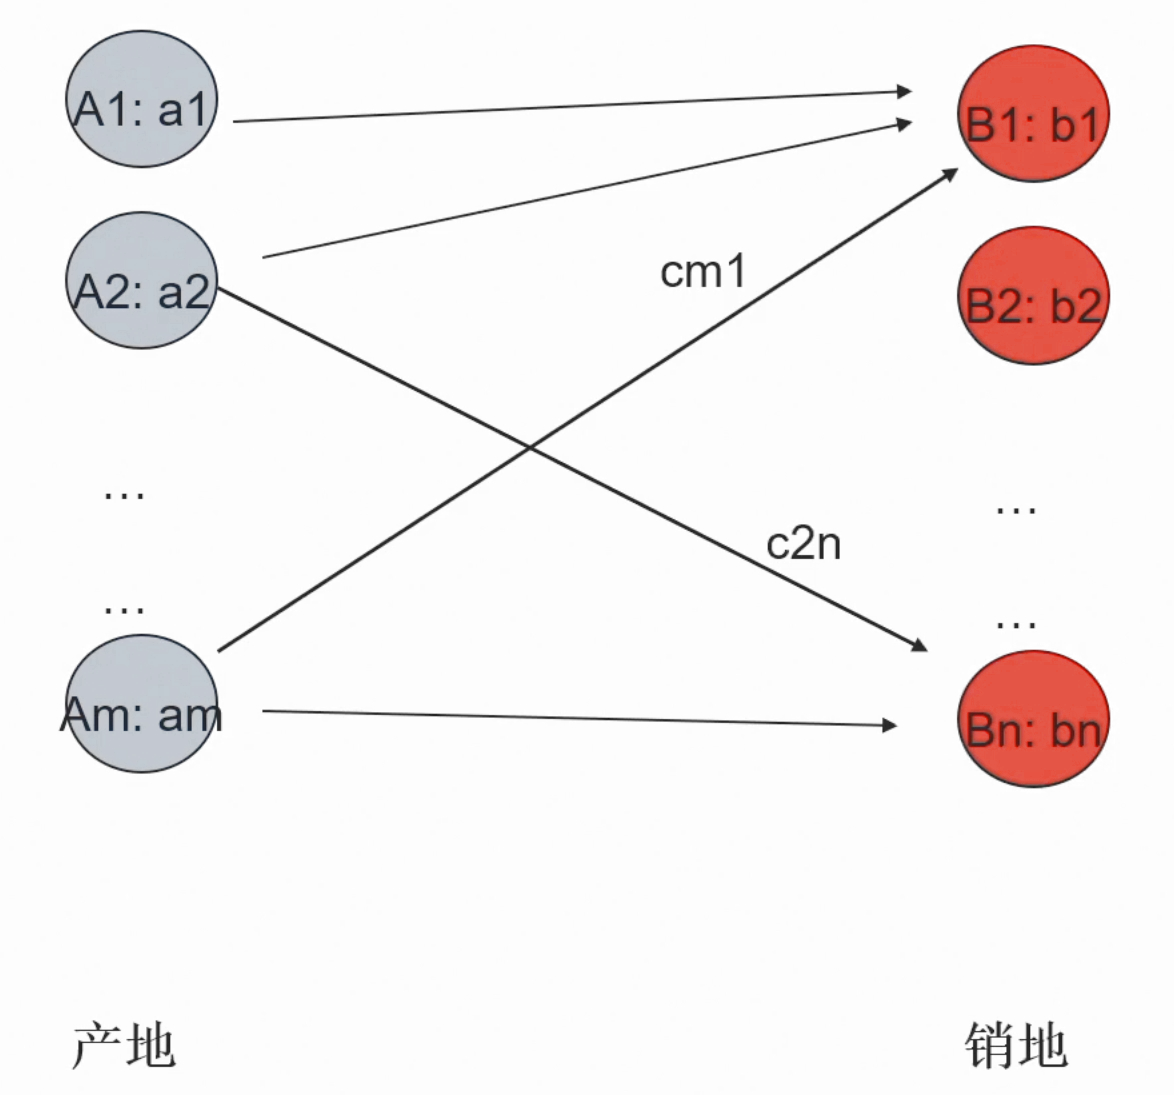
\includegraphics[width=0.6\textwidth]{5.png}
    \caption{例1.1.3图解}
    \label{fig:Temporary Pavilion}
\end{figure}
优化目标为最小化总运费,数学模型如下:

\begin{equation}
\min z = \sum_{i=1}^{m} \sum_{j=1}^{n} c_{ij} x_{ij}
\end{equation}

约束条件:
\begin{align}
&\sum_{j=1}^{n} x_{ij} = a_i, \quad i = 1, 2, \dots, m \tag{m 个约束方程} \\
&\sum_{i=1}^{m} x_{ij} = b_j, \quad j = 1, 2, \dots, n \tag{n 个约束方程} \\
&x_{ij} \geq 0, \quad i = 1, 2, \dots, m; \, j = 1, 2, \dots, n \tag{m $\times$ n 个变量}
\end{align}

约束条件的系数矩阵共 $m + n$ 行,$m \times n$ 列的矩阵,即 $x_{ij}$ 的系数向量。

\begin{equation}
\mathbf{p_{ij}} = (0, \dots, 1, \dots, 1, \dots, 0)^{\top}, \quad i \text{ 行, } m+j \text{ 行}
\end{equation}

分量中除第 $i$ 个和第 $m+j$ 个元素为 1,其余均为 0。
\\
关于产销平衡的运输问题,还有
\begin{equation}
\sum_{i=1}^{m} a_i = \sum_{i=1}^{m} \left( \sum_{j=1}^{n} x_{ij} \right) = \sum_{j=1}^{n} \left( \sum_{i=1}^{m} x_{ij} \right) = \sum_{j=1}^{n} b_j \,,
\end{equation}

所以模型中最多有 $m+n-1$ 个独立约束方程,即系数矩阵的秩不超过 $m+n-1$\footnote{原本有$m+n$个方程,但是根据题目中提到的“产销平衡”,可以列出方程3.3,即自由度减1,消去了一个约束,可行域增大}。
\end{exbox}

\subsection{产销不平衡}
事实上,我们知道,市场上几乎不可能出现“产销平衡”的情况,供大于求(产大于销)、供不应求(销大于产)的情况更为常见。
\textcolor{red}{产销不平衡问题一般都是转化为产销平衡问题解决的。}
\begin{exbox}{\textbf{产销不平衡的运输问题}}
    1
    \begin{enumerate}
        \item[(1)] \textbf{产大于销时:}
        
        由于
        \begin{equation}
            \sum_{j=1}^{n} b_j < \sum_{i=1}^{m} a_i \,,
        \end{equation}
        
        则问题的模型为
        \begin{equation}
            \min z = \sum_{i=1}^{m} \sum_{j=1}^{n} c_{ij} x_{ij} \,,
        \end{equation}
        
        约束条件:
        \begin{align}
            \sum_{j=1}^{n} x_{ij} &\leq a_i \quad i=1,2,\dots,m \,, \\
            \sum_{i=1}^{m} x_{ij} &= b_j \quad j=1,2,\dots,n \,, \\
            x_{ij} &\geq 0 \quad i=1,2,\dots,m;\ j=1,2,\dots,n \,.
        \end{align}
        其中,$\sum_{j=1}^{n} x_{ij} \leq a_i$ 表示 $i$ 产品的总产量小于或等于其产量。
        \\
        \item[(2)] \textbf{销大于产时:}
        
        由于
        \begin{equation}
            \sum_{j=1}^{n} b_j > \sum_{i=1}^{m} a_i \,,
        \end{equation}
        
        则问题的数学模型为
        \begin{equation}
            \min z = \sum_{i=1}^{m} \sum_{j=1}^{n} c_{ij} x_{ij} \,,
        \end{equation}
        
        约束条件:
        \begin{align}
            \sum_{j=1}^{n} x_{ij} &= a_i \quad i=1,2,\dots,m \,, \\
            \sum_{i=1}^{m} x_{ij} &\leq b_j \quad j=1,2,\dots,n \,, \\
            x_{ij} &\geq 0 \quad i=1,2,\dots,m;\ j=1,2,\dots,n \,.
        \end{align}
        其中,$\sum_{i=1}^{m} x_{ij} \leq b_j$ 表示 $i$ 产品的总产量小于或等于其销量。
    \end{enumerate}
    
    此时,要将各约束资源
    \begin{equation}
        \sum_{i=1}^{m} a_i - \sum_{j=1}^{n} b_j = b_{n+1} \,,
    \end{equation}
    
    在生产地或销地储存起来,即使没有一个虚拟的销售地,其运费为零,即设 $x_{i,n+1}$ 表示产地 $A_i$ 多年产(需要储存)的物资数量,运费为 $c_{i,n+1}=0$ $(i=1,2,\dots,m)$,其目标函数不变。于是问题的模型变为
    \begin{equation}
        \min z = \sum_{i=1}^{m} \sum_{j=1}^{n} c_{ij} x_{ij} \,,
    \end{equation}
    
    约束条件:
    \begin{align}
        \sum_{j=1}^{n} x_{ij} + x_{i,n+1} &= a_i \quad (i=1,2,\dots,m) \,, \label{eq:balance1} \\
        \sum_{i=1}^{m} x_{ij} &= b_j \quad (j=1,2,\dots,n) \,, \label{eq:balance2} \\
        \sum_{i=1}^{m} x_{i,n+1} &= \sum_{i=1}^{m} a_i - \sum_{j=1}^{n} b_j = b_{n+1} \,, \label{eq:balance3} \\
        x_{ij}, x_{i,n+1} &\geq 0 \quad (i=1,2,\dots,m;\ j=1,2,\dots,n) \,. \label{eq:nonneg}
    \end{align}
    公式 \eqref{eq:balance1} 表示转化为产销平衡问题。
\end{exbox}
\begin{figure}[H]
    \centering
    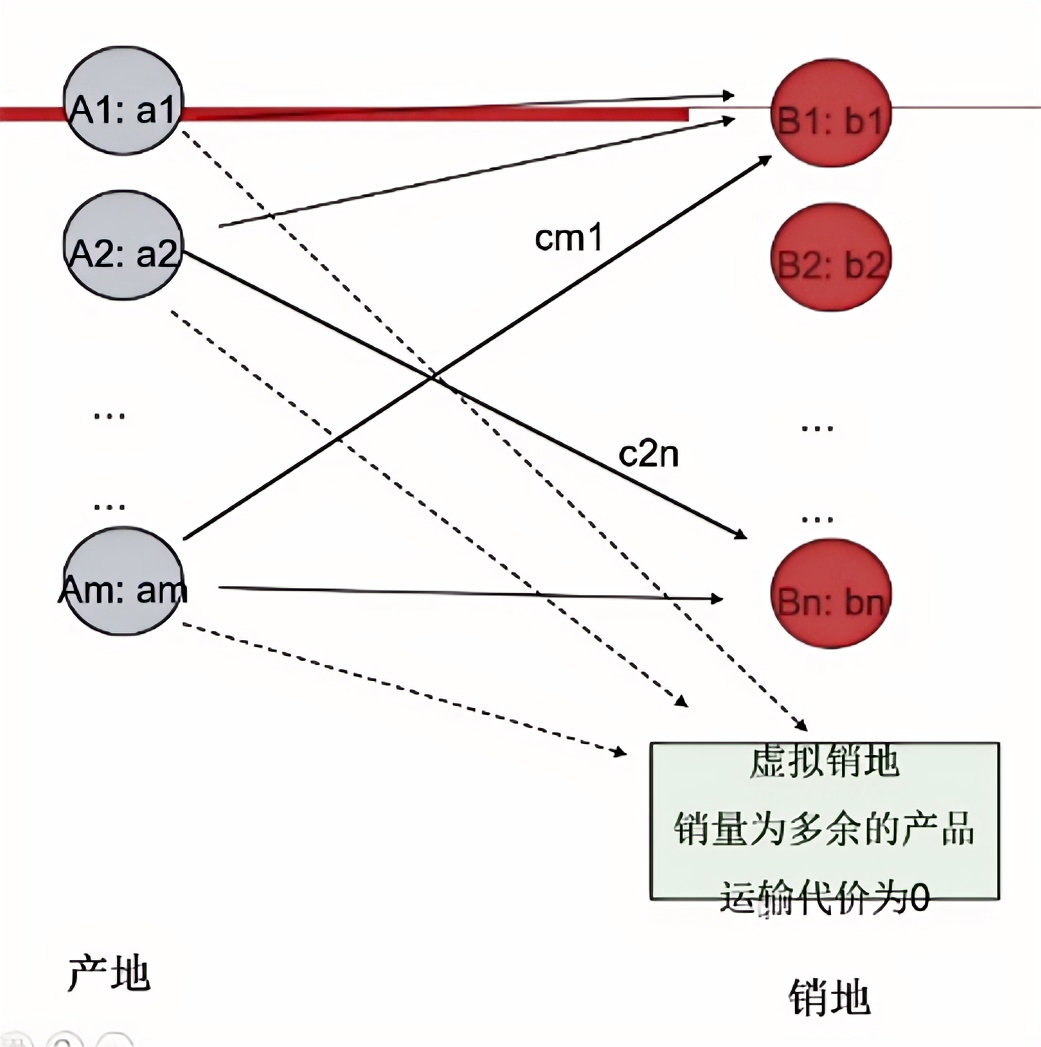
\includegraphics[width=0.5\textwidth]{6.png}
    \caption{产大于销的情况}
    \label{fig:Temporary Pavilion}
\end{figure}

\begin{figure}[H]
    \centering
    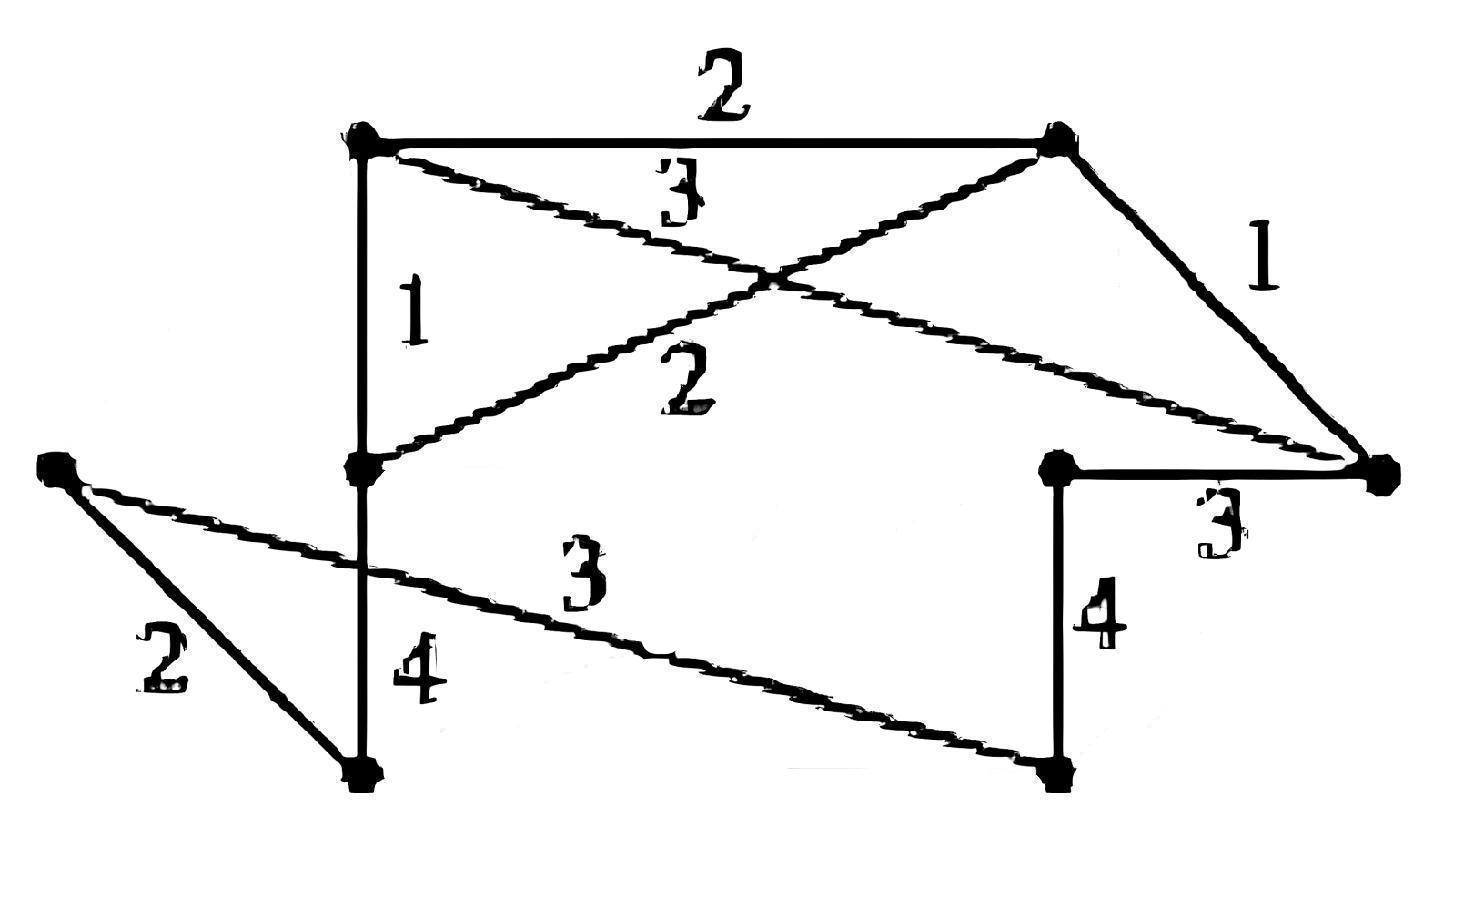
\includegraphics[width=0.5\textwidth]{7.png}
    \caption{销大于产的情况}
    \label{fig:Temporary Pavilion}
\end{figure}

\ifx\allfiles\undefined
	
	% 如果有这一部分的参考文献的话,在这里加上
	% 没有的话不需要
	% 因此各个部分的参考文献可以分开放置
	% 也可以统一放在主文件末尾。
	
	%  bibfile.bib是放置参考文献的文件,可以用zotero导出。
	% \bibliography{bibfile}
	
	end{document}
	\else
	\fi